\documentclass{article}
% translate with >> pdflatex -shell-escape <file>

% This file is an extract of the PGFPLOTS manual, copyright by Christian Feuersaenger.
% 
% Feel free to use it as long as you cite the pgfplots manual properly.
%
% See
%   http://pgfplots.sourceforge.net/pgfplots.pdf
% for the complete manual.
%
% Any required input files (for <plot table> or <plot file> or the table package) can be downloaded
% at
% http://www.ctan.org/tex-archive/graphics/pgf/contrib/pgfplots/doc/latex/
% and
% http://www.ctan.org/tex-archive/graphics/pgf/contrib/pgfplots/doc/latex/plotdata/

\usepackage{pgfplots}
\pgfplotsset{compat=newest}

\pagestyle{empty}

\begin{document}
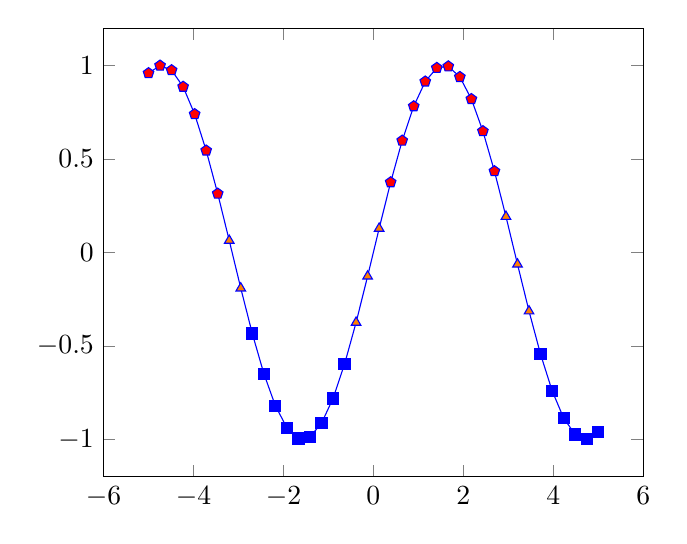
\begin{tikzpicture}
% Low-Level scatter plot interface Example: 
% use three different marker classes 
% 0% - 30%   : first class
% 30% - 60%  : second class
% 60% - 100% : third class
\begin{axis}[
scatter/@pre marker code/.code={%
   \ifdim\pgfplotspointmetatransformed pt<300pt
      \def\markopts{mark=square*,fill=blue}%
   \else
      \ifdim\pgfplotspointmetatransformed pt<600pt
         \def\markopts{mark=triangle*,fill=orange}%
      \else
         \def\markopts{mark=pentagon*,fill=red}%
      \fi
   \fi
   \expandafter\scope\expandafter[\markopts]
},%
scatter/@post marker code/.code={%
   \endscope
}]

\addplot+[scatter,scatter src=y,
	samples=40]
   {sin(deg(x))};
   
\end{axis}
\end{tikzpicture}
\end{document}
